\documentclass[12pt, usenatbib]{article}
\usepackage{aas_macros}
\usepackage{graphicx,color}
\usepackage[margin=0.75in]{geometry}
\usepackage{amssymb}
\usepackage{footnote, enumerate, url, amsmath}
\usepackage{natbib}
\usepackage{multirow, multicol}
\setlength\columnsep{30pt}
\usepackage{tabularx}
\usepackage{hyperref}
\usepackage{amssymb}
\usepackage{setspace}

\hypersetup{
    colorlinks,
    citecolor=black,
    filecolor=black,
    linkcolor=black,
    urlcolor=black
}

\usepackage{titling}
\newcommand{\subtitle}[1]{%
  \posttitle{%
    \par\end{center}
    \begin{center}\large#1\end{center}
    \vskip0.5em}%
}

\def\starpy {\textsc{starpy}}


\begin{document}

\title{Summary of PhD Research}
\subtitle{\emph{The influence of morphology, AGN and environment on the quenching histories of galaxies}}
\author{Rebecca Smethurst}

\maketitle


What drives the evolution of galaxies from the disc dominated, star forming blue cloud to the elliptical dominated, quiescent red sequence? What role does the morphology, central supermassive black hole and galaxy environment play in this shut down of star formation? 
% How do you answer them? STARPY?

In my thesis, I attempted to answer these questions by using Bayesian statistics to infer a simple star formation history (SFH) describing the time, $t_q$, and exponential rate, $\tau$, that star formation shuts down (referred to as quenching) in a galaxy. This statistical approach allowed me to reveal the subtle morphologically dependent evolutionary pathways taken between the blue cloud and red sequence by galaxies of all shapes and environments. Galaxies lying within the sparsely populated colour space between these two populations are dubbed as `green valley' galaxies, which have long been thought of as the `crossroads' of galaxy evolution. Previous studies have suggested that the evolution of galaxies through the `green valley' is purely bimodal, with elliptically shaped galaxies quenching rapidly and disc galaxies quenching slowly. In my thesis however, I was able to infer a broad range of quenching rates occurring across the galaxy population for a diverse range of morphologies. 

This was possible due to classifications from Galaxy Zoo, a citizen science project enlisting the help of thousands of members of the public to voluntarily classify galaxy images online\footnote{\url{http://galaxyzoo.org}}. The project has produced highly accurate and robust detailed morphological classifications and is a significant statistical improvement over efforts completed using only a small number of expert classifiers \citep[e.g.][]{schawinski07, nair10b, ann15}. 

The classifications from volunteers produces a vote fraction for each galaxy; for example a disc vote fraction of $p_{d} = 0.8$. The vote fractions encompass the continuous spectrum of morphological features (as shown in Figure~\ref{fig:mosaic}), rather than a simple binary classification separating smooth and disc galaxies as used by previous studies \citep{ravindranath04, kelvin12, schawinski14, vika15}. These classifications allow each galaxy to be considered as a probabilistic object with both bulge and disc components. I believe that it is this novel implementation of the morphological classifications that has allowed me to discover the subtle differences in quenching histories for galaxies of different morphologies in this thesis. 

\begin{figure}[t]
\centering{
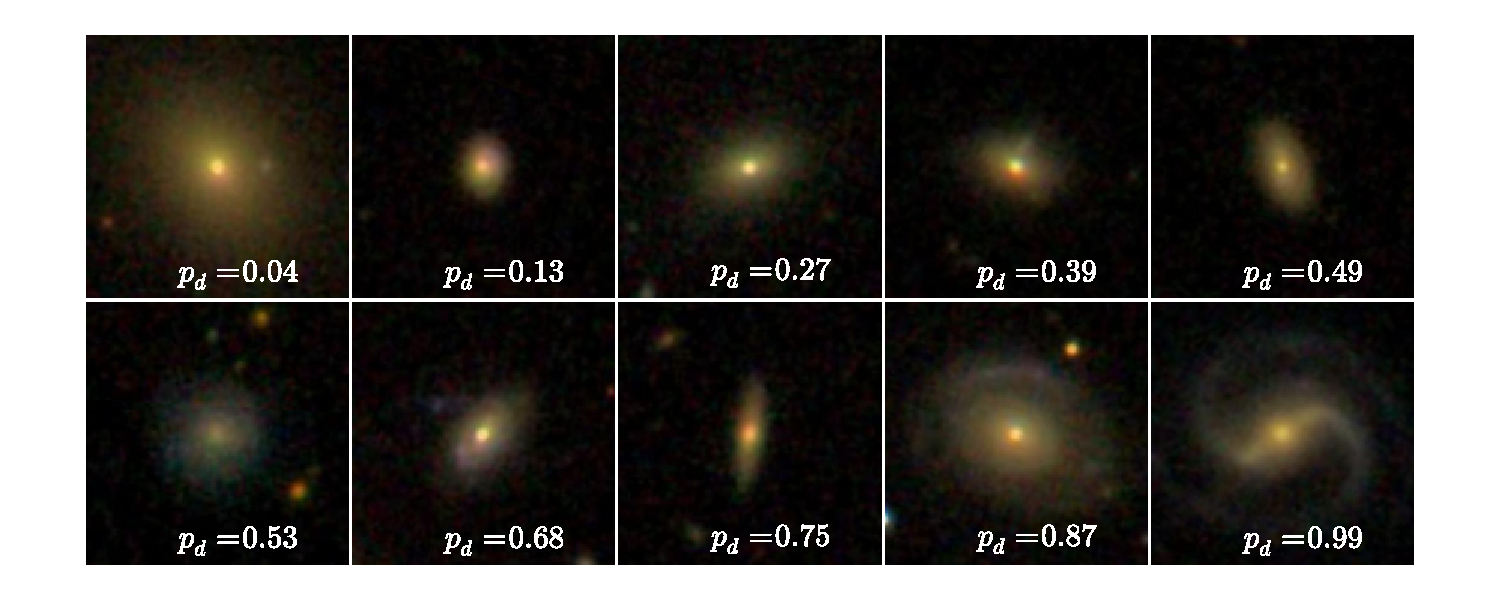
\includegraphics[width=\textwidth]{mosaic_disc_fraction_z_0-07_0-075.pdf}}
\caption{Randomly selected SDSS $gri$ composite images showing the continuous probabilistic nature of the Galaxy Zoo classifications for galaxies in a redshift range $0.070 < z < 0.075$. The disc vote fraction for each galaxy is shown. The scale for each image is $0.099~\rm{arcsec/pixel}$.}
\label{fig:mosaic}
\end{figure}

In order to infer the SFH of a single galaxy, I used the optical photometry, provided by the Sloan Digital Sky Survey (SDSS), and the near ultra-violet (NUV) photometry, from the GALEX survey, in order to infer the posterior distribution across the two dimensional $[t_q, \tau]$ parameter space. I then utilised the Galaxy Zoo 2 morphological classifications to obtain a morphology weighted (either weighted by their disc vote fraction or smooth vote fraction), combined population distribution across each quenching parameter for a sample of galaxies. 
% What do you find in morph chapter?

I applied this method across the blue cloud, green valley and red sequence within a sample of $126,316$ galaxies and found a clear difference between the quenching timescales preferred by smooth and disc weighted populations, with three major routes through the green valley dominated by smooth (rapid rates, attributed to major mergers), intermediately classified (intermediate rates, attributed to galaxy interactions) and disc morphologies (slow rates, attributed to secular, i.e. slow, processes). I hypothesised that morphological changes occur in systems which have undergone quenching with an exponential rate, $\tau < 1.5~\rm{Gyr}$, in order for the evolution of galaxies in the green valley to match the ratio of smooth to disc galaxies observed in the red sequence.
% What do you find in AGN feedback chap?

Along with the morphological dependence of galaxy evolution, the active central supermassive black hole of a galaxy (an active galactic nucleus; AGN) is thought to affect a galaxy's star formation rate in a process known as AGN feedback. AGN feedback was first suggested as a mechanism for regulating star formation due to the results of simulations wherein galaxies could grow to unrealistic stellar masses. This stellar mass build up is thought to occur through many mergers of galaxies over cosmic time, a process which AGN feedback can regulate by either rapidly expelling or heating the gas needed for further star formation, causing a quench and reducing the ultimate stellar mass of a galaxy. So far, only indirect observational evidence has been found for AGN feedback, the strongest being the indirect evidence that the largest AGN fraction is found in the green valley \citep{cowie08, hickox09, schawinski10}, suggesting a link between AGN activity and the process which moves a galaxy from the blue cloud to the red sequence.

I therefore repeated my SFH analysis for a sample of $1,244$ obscured AGN host galaxies and found statistical evidence for recent, rapid quenching, suggesting that this may be caused by AGN feedback. This result is shown by the population distributions shown in Figure~\ref{fig:agnfeedback}. This result is the first statistically supported observational evidence for AGN feedback in a population of galaxies. 

\begin{figure*}[t]
\centering{
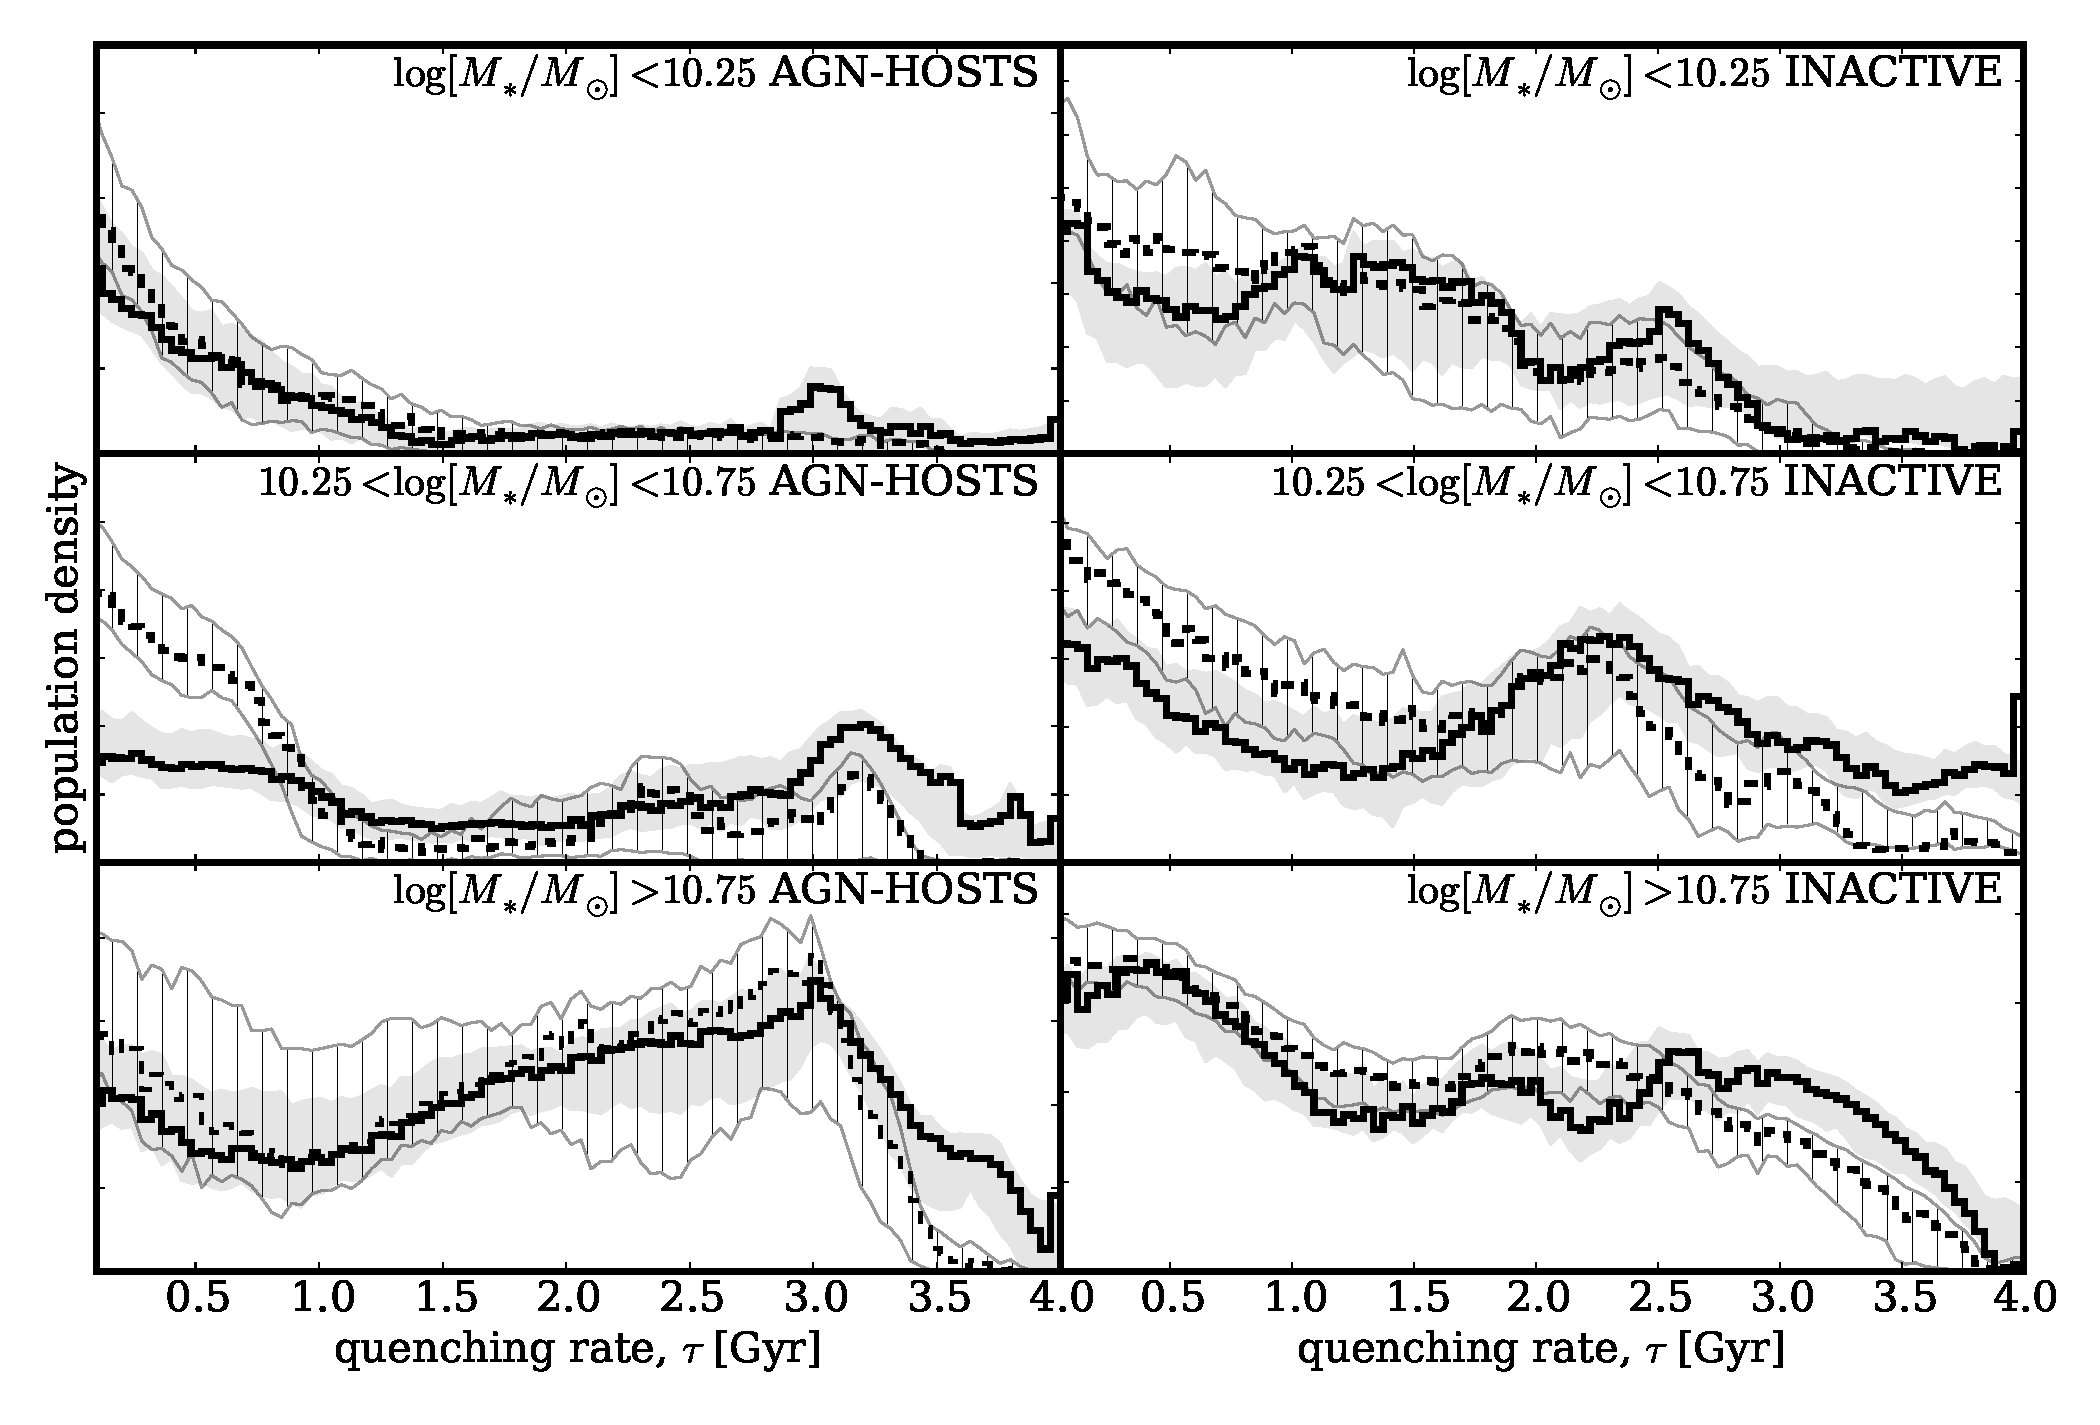
\includegraphics[width=\textwidth]{fig5.pdf}}
\caption{Population density distributions showing the rate that quenching occurs ($\tau$) for AGN host galaxies (left) and those not hosting an AGN (inactive galaxies; right), which are split into low (top), medium (middle) and high (bottom) stellar mass. Each population is weighted by both the smooth (dashed line) and disc (solid line) morphology classifications from Galaxy Zoo. Uncertainties  are shown by the shaded regions for the smooth (grey striped) and disc (grey solid) population densities. A small value of $\tau$ corresponds to a rapid quench.}
\label{fig:agnfeedback}
\end{figure*}

However, Figure~\ref{fig:agnfeedback} also shows that rapid quenching rates cannot account for all the quenching across the AGN host population; slow quenching rates, attributed to secular evolution, are also significant in the evolution of AGN host galaxies. This is contrary to many previous works suggesting that the bulk of galaxy-black hole co-evolution occurs in violent processes such as mergers which simultaneously grow both the black hole and galaxy, and in particular the central stellar bulge component of a galaxy. Conversely, slow secular processes are not theorised to be able to significantly grow the black hole such that it has enough energy to cause feedback on its host galaxy.
% What do you find in bulgeless AGN?

I investigated this possible secular co-evolution of galaxies and black holes further in my thesis by measuring the black hole masses of a sample of $101$ bulgeless AGN host galaxies. Bulgeless galaxies are thought to arise due to a lack of bulge building mergers in a galaxy's evolutionary history. I compared the black hole masses of these bulgeless galaxies to those of typical galaxies and compared their locations on well known black hole-galaxy scaling relations, as shown in Figure~\ref{fig:bulgevsbh}. I found that the measured black holes of the bulgeless galaxies are $10-100$ times more massive than they should be, given their lack of bulges. However, I also found that the measured black holes of these bulgeless galaxies adhere to the typical correlation found with total stellar mass of their host galaxies. The results in this thesis therefore suggest that black hole-galaxy scaling relations may arise due to mutual correlations to the overall gravitational potential of the dark matter halo of the galaxy, contradicting the long held theory that black holes only grow to large masses during galaxy mergers. 

\begin{figure*}[t]
\centering
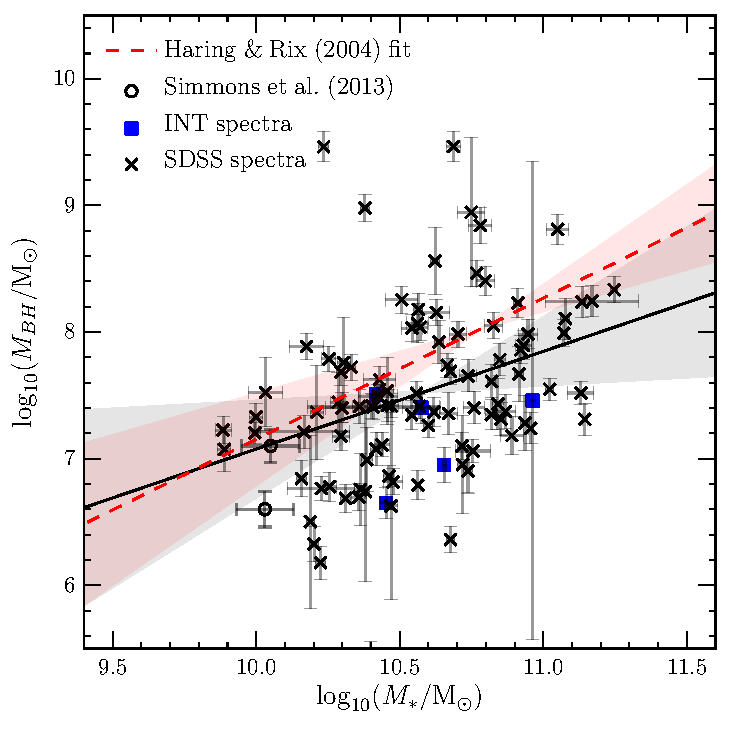
\includegraphics[width=0.48\textwidth]{mass_bh_total_mass_fit_linmix_fit.pdf}
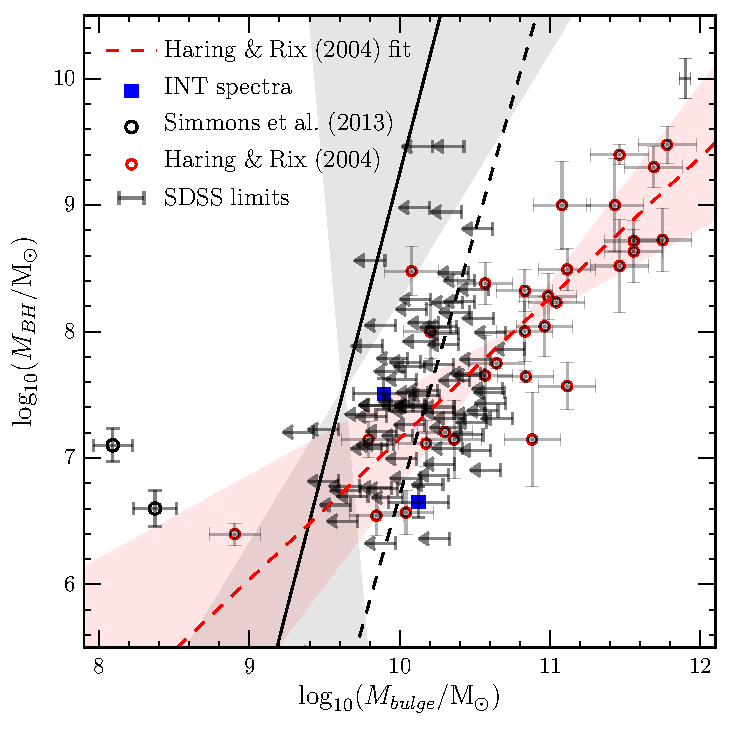
\includegraphics[width=0.48\textwidth]{mass_bh_bulge_limits_INT_simmons13_measurements_linmix_fit.pdf}
\caption{(a) Total stellar mass against the black hole mass of the 101 bulgeless galaxies (crosses and blue squares) with two bulgeless galaxy measurements from Simmons et al. (2013; open circles) also shown. The best fit line to the data points and two-dimensional errors from linear regression is shown (solid line) with $\pm3\sigma$ (grey shaded). I also show the best fit found using this same method to the typical bulge dominated galaxies of \protect\citet[][dashed line]{haringrix04} with $\pm3\sigma$ (red shaded). (b) The upper limits on the calculated stellar bulge masses are plotted against the black hole mass for the 101 bulgeless galaxies. The best fit to these upper limits and two-dimensional errors using linear regression methods (solid line) is shown with $\pm3\sigma$ (grey shaded). The dashed line shows the fit if the upper limits are not treated as such. I also show the best fit found using this same method to the typical bulge dominated galaxies of \protect\citet[][dashed line]{haringrix04} with $\pm3\sigma$ (red shaded).
}
\label{fig:bulgevsbh}
\end{figure*}
% What do you find in environment chapter?

I also considered the effect of the group environment on the time and rate that quenching occurs. The galaxy environment as a driver of quenching was proposed due to the fact that star forming disc galaxies tend to be located in low-density environments, such as voids and the satellites of small groups, with quiescent galaxies in more dense environments, such as the central galaxies of large groups and clusters. The most likely (and therefore the most studied) candidate mechanism for the cause of this environmental correlation is ram pressure stripping \citep{abadi99, poggianti99}. However, there has been mounting evidence that RPS can only strip a galaxy of $40-60\%$ of its gas supply \citep{fillingham16} and so may not be as effective a quenching mechanism as first thought \citep{emerick16}. Therefore although the correlation of a galaxy's environment with it's morphology and star formation rate were originally interpreted as indicating causation, recent evidence from simulations suggests that quenching mechanisms driven by the environment may not be dominant in the galaxy lifecycle \citep{kimm11, hirschmann14, wang14, phillips15}.

In my thesis I studied the effect on the quenching rate for group galaxies with respect to their group-centric radius, for $4,629$ satellite galaxies using my SFH inference method. I found that although many different mechanisms are all occurring in groups, such as mergers and secular processes, environmentally driven quenching mechanisms are also prevalent. However, I find that these environmentally driven quenching processes are not correlated with the velocity of a satellite within a group, ruling out ram pressure stripping as the dominant environmental quenching mechanism, in agreement with results from recent simulations \citep{fillingham16, emerick16}. 
% Sum up your big picture

My thesis concluded with an in-depth discussion detailing how there are many quenching mechanisms which will act upon a galaxy over its lifetime, rather than a single dominant mechanism as is often sought after in the literature \citep[e.g.][]{muzzin12, schawinski14, foltz15, woo15, balogh16, darvish16, huertascompany16}. Instead many quenching mechanisms are likely to act in concert to reduce the SFR, which in turn produces the wide distribution of quenching rates seen across the galaxy population in this thesis. 

I also discussed ideas for future work adapting the inference method introduced in this thesis to take spectral information (rather than photometric data) as inputs with which to infer the SFH of a galaxy. During my current role as a research fellow, I am applying this addated method to data from the MaNGA IFU survey \citep{bundy15}, which takes up to $127$ individual fibre spectra observations across the extent of a galaxy, rather than a single global galaxy spectrum as in previous surveys. 

The adapted SFH inference method developed for the work in this thesis combined with the plethora of new data from the MaNGA survey will allow the spatial extent of quenching in a galaxy to be studied, revolutionising our understanding of the processes which cause the transition of a galaxy from star forming to quiescent. In particular I aim to follow up on my result showing statistical evidence for AGN feedback occurring in a population of AGN host galaxies, to determine how this process occurs. Specifically, does the AGN heat or expel the gas needed for star formation in a galaxy? This should be discernible in the spatially mapped inferred quenching history of a galaxy derived by my adapted inference method.  

\begin{thebibliography}{}
\small
\begin{multicols}{2}
\setstretch{0.5}
\bibitem[\protect\citeauthoryear{Abadi, Moore \& Bower}{1999}]{abadi99} Abadi M. G., Moore B. \& Bower R. G., 1999, MNRAS, 308, 947
\bibitem[\protect\citeauthoryear{Ann et al.}{2015}]{ann15} Ann H. B., Seo M., Ha D. K., 2015, ApJS, 217, 27
\bibitem[\protect\citeauthoryear{Balogh et al.}{2016}]{balogh16} Balogh M. L. et al., 2016, MNRAS, 456, 4364
\bibitem[\protect\citeauthoryear{Bundy et al.}{2015}]{bundy15} Bundy K. et al., 2015, ApJ, 798, 7   
\bibitem[\protect\citeauthoryear{Cowie \& Barger}{2008}]{cowie08} Cowie L. L., Barger A. J., 2008, ApJ, 686, 72
\bibitem[\protect\citeauthoryear{Darvish et al.}{2016}]{darvish16} Darvish B. et al., 2016, ApJ, 825, 113
\bibitem[\protect\citeauthoryear{Emerick et al.}{2016}]{emerick16} Emerick A. et al., 2016,ApJ, 826, 148
\bibitem[\protect\citeauthoryear{Fillingham et al.}{2016}]{fillingham16} Fillingham S. P. et al., 2016, MNRAS, 463, 1916
\bibitem[\protect\citeauthoryear{Foltz et al.}{2015}]{foltz15} Foltz R. et al., 2015, ApJ, 812, 138
\bibitem[\protect\citeauthoryear{Haring \& Rix}{2004}]{haringrix04} H\"aring N., Rix H.-W., 2004, ApJ, 604, L89
\bibitem[\protect\citeauthoryear{Hickox et al.}{2009}]{hickox09} Hickox R. C. et al., 2009, ApJ, 696, 891
\bibitem[\protect\citeauthoryear{Hirschmann et al.}{2014}]{hirschmann14} Hirschmann M. et al., 2014, MNRAS, 444, 2938
\bibitem[\protect\citeauthoryear{Huertas-Company et al.}{2016}]{huertascompany16} Huertas-Company M. et al., 2016, MNRAS, 462, 4495
\bibitem[\protect\citeauthoryear{Kelvin et al.}{2012}]{kelvin12} Kelvin L. S. et al., 2012, MNRAS, 421, 1007
\bibitem[\protect\citeauthoryear{Kim, Yi \& Khochfar}{2011}]{kimm11} Kimm T., Yi S. K., Khochfar S., 2011, ApJ, 729, 11
\bibitem[\protect\citeauthoryear{Muzzin et al.}{2012}]{muzzin12} Muzzin A. et al., 2012, ApJ, 746, 188
\bibitem[\protect\citeauthoryear{Nair \& Abraham}{2010}]{nair10b} Nair, P. B. \& Abraham, R. G. 2010, ApJSS, 186, 427
\bibitem[\protect\citeauthoryear{Phillips et al.}{2015}]{phillips15} Phillips J. I. et al., 2015, MNRAS, 447, 698
\bibitem[\protect\citeauthoryear{Poggianti et al.}{1999}]{poggianti99} Poggianti B. M. et al., 1999, ApJ,
518, 576
\bibitem[\protect\citeauthoryear{Ravindranath et al.}{2004}]{ravindranath04} Ravindranath S. et al., 2004, ApJ, 604, L9
\bibitem[\protect\citeauthoryear{Schawinski et al.}{2007}]{schawinski07} Schawinski, et al., 2007, MNRAS, 382, 1415
\bibitem[\protect\citeauthoryear{Schawinski et al.}{2010}]{schawinski10} Schawinski K. et al., 2010, ApJ, 711, 284
\bibitem[\protect\citeauthoryear{Schawinski et al.}{2014}]{schawinski14} Schawinski, K. et al., 2014, MNRAS, 440, 889
\bibitem[\protect\citeauthoryear{Vika et al.}{2015}]{vika15} Vika M. et al., 2015, A\&A, 577, A97
\bibitem[\protect\citeauthoryear{Wang et al.}{2014}]{wang14} Wang W. et al., 2014, MNRAS, 442, 1363
\bibitem[\protect\citeauthoryear{Woo et al.}{2015}]{woo15} Woo J. et al., 2015, MNRAS,
448, 237

\end{multicols}
\end{thebibliography}

\end{document}